\documentclass[border=1pt]{standalone}
\usepackage[dvipsnames]{xcolor}
\usepackage{tikz}                       % Graphen und kommutative Diagramme
\usetikzlibrary{patterns}               % Um schraffierte Formen in der tikzpicture-Umgebung zu zeichnen.
\newcommand{\ul}[1]{\underline{\smash{#1}}}

\begin{document}

\centering
\resizebox{!}{4cm}{
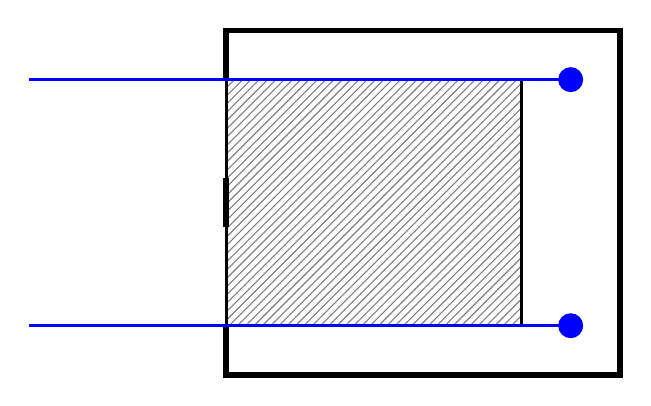
\begin{tikzpicture}[x=1.25cm, y=1.25cm, line width=1pt]
    % draw outer lines
    \draw (0, 0) -- (4, 0) -- (4, 3.5) -- (0, 3.5) -- (0, 0);
    
    % draw shaded slit box
    \filldraw[pattern=north east lines, pattern color=black!50] (0, 0.5) -- (3, 0.5) -- (3, 3) -- (0, 3) -- (0, 0.5);
    
    % draw line width=2pt boundary lines
    \draw[line width = 2pt] (0, 0.5) -- (0, 0) -- (4, 0) -- (4, 3.5) -- (0, 3.5) -- (0, 3);
    \draw[line width = 2pt] (0, 1.5) -- (0, 2);
    
    % draw slits
    \draw[color=blue, line width=1.2pt] (-2, 0.5) -- (3.5, 0.5);
    \draw[color=blue, line width=1.2pt] (-2, 3) -- (3.5, 3);
    \filldraw[fill = blue, draw = blue] (3.5, 0.5) circle (4pt);
    \filldraw[fill = blue, draw = blue] (3.5, 3)   circle (4pt);

\end{tikzpicture}
}

\end{document}
